\subsection{Development View}

Our development view is represented through a package diagram, and gives a brief overview of the different packages implemented in GAPP and CAPP. 
We have implemented somewhere around 120 different Java classes, which does not include the Karotz code. 

\subsubsection{Development View -- GAPP}
\label{sec:gapp-dev-view}

\begin{figure}
	\centering
		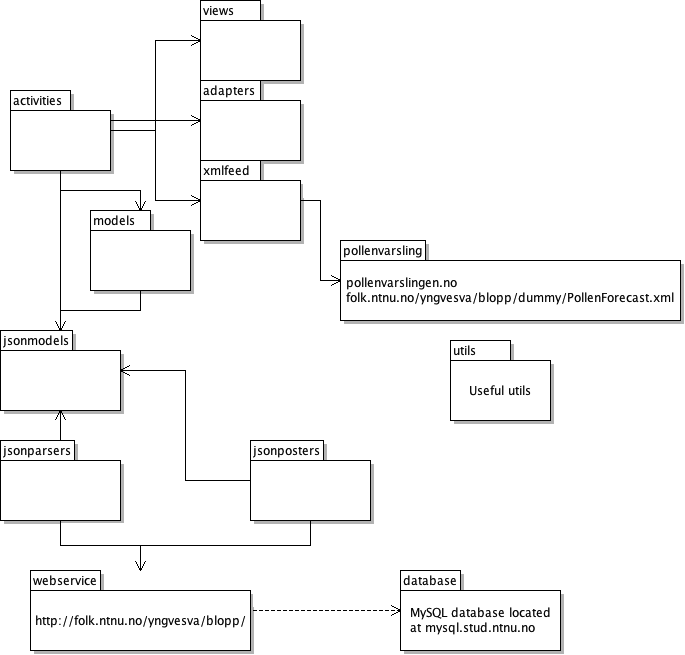
\includegraphics[width = 11.5 cm]{Pictures/ArchPictures/gapparchpictures/gapp_package_diagram.png}
	\caption[GAPP package diagram]{Package diagram for GAPP. A line from package X to package Y describes an association from X to Y. }
	\label{fig:package-diagram-gapp}
\end{figure}

Figure \ref{fig:package-diagram-gapp} show the top level package structure for GAPP. In the logical view, we introduced our webservice. 
From this webservice, we retrieve data over HTTP GET,
using JSON (JavaScript Object Notation). The classes found in jsonposters uses HTTP POST to send data to the webservice, which in turn forwards the information sent to our database. 

The diagram also shows a package called xmlfeed. This package serves the purpose of parsing XML (Extensible Markup Language) into Java-code. Originally, the idea was to
use NAAF's XML-feed. However, this feed is not running during autumn and winter, so we replicated that XML-feed in our own
``dummy''-feed \footnote{This XML-file is hosted at: \url{http://folk.ntnu.no/yngvesva/blopp/dummy/PollenForecast.xml}}. 
This xml-document has similar structure as the original feed, only with test data for the sake of the prototype and proof-of-concept.

The package activities contains classes that extends \code{Activity}, which is an android class that functions as both the View and Controller in MVC. 
An example of an implemented activity is \code{MainMenu}.

In order to render listviews and gridviews programatically, we needed to make a package called adapters. An \code{Adapter} in Android serves the purpose of filling  
these list- and gridviews with data.
 
Views in Android can be created in two ways. Either through an XML layout file, or by customising in Java. Most of our views are using XML-files. We have one custom
made view (\code{CalendarView}, used to implement our logging functionality), which is available in the package ``views''. 
The XML-files are not shown in this diagram, but is included in the application's resource folder, which is standard when working
in the Android framework.  
  

We'll explain the content in each package more detailed in the Development View.

\subsubsection{Development View -- CAPP}
\begin{figure}
	\centering
		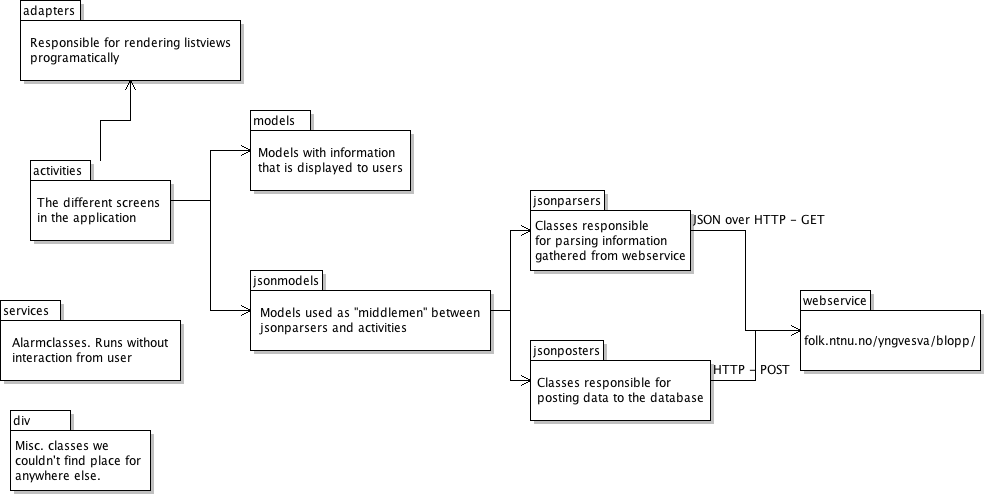
\includegraphics[width = 11.5 cm]{Pictures/ArchPictures/capparchpictures/capp_package_diagram}
	\caption[GAPP package diagram]{Package diagram for CAPP. A line from package X to package Y describes an association from X to Y. }

	\label{fig:package-diagram-system-capp}
\end{figure}

Figure \ref {fig:package-diagram-system-capp} shows the package diagram for CAPP. CAPP has very similar architecture as GAPP.
The main difference is the ``services'' package. A service in Android is a task that is executed without any interactions from the user. In our case,
we use the services-package to update alarms. CAPP uses the same database and webservice as GAPP, and
a lot of the parsers in this application are equal to those found in GAPP.

\subsubsection{Development View -- Karotz}
 \begin{figure}
 	\centering
 		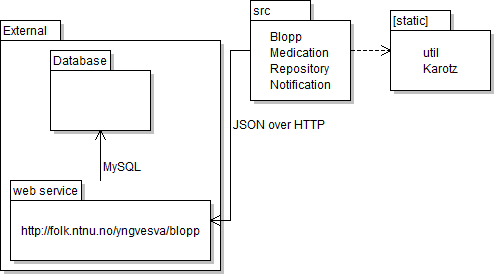
\includegraphics[width=12cm]{Pictures/ArchPictures/KarotzPackageDiagram}
	\caption[Karotz package diagram]{Package diagram for the Karotz application}
	\label{fig:package-diagram-system-karotz}
 \end{figure}

Figure \ref{fig:package-diagram-system-karotz} shows the development view of the Kartoz application. The only internal package in the Karotz application
is named ``src''. It contains all the main logic for the application, including a repository for connecting to the webservice for connecting to the
database, a notification module for setting alarms, a medication module for doing distraction, and a ``Blopp'' module for keeping track of everything.
There is an additional package in the diagram named ``\lbrack{}static\rbrack{}''. It contains the Karots class which is inherited from the OS and
contains various utilities for controlling output and recieveing input for the robot. It has been extended with some helper methods in the
implementation. There is also a ``util'' class which contains additional utility methods that do not belong in ``Karotz''. At last, there is indicated
an ``External'' package, which symbolizes all the external services the application connects to. In the case of the Karotz application, this includes
only the web service that connects to the database.